
\chapter{Platform design}
\label{ch:ch4}

In this chapter, the hardware design processes are outlined based on the user requirements and technical specifications given in Chapter \ref{ch:ch3}. This chapter begins with a description of the mechanical features showing how the design accommodates the electronic subsystems while meeting the functional requirements outlined in Table \ref{tab:hard_funcreqsl}. This chapter then shows the electronic components selected for each subsystem and how they affect the overall system. Finally, this chapter will conclude with the final design considerations for the buoy. \par 

Son and Vorajee in 2018 performed initial concept work for the buoy, which strongly influenced the current design choices for this device. Furthermore, MacHutchon designed the original buoy stand with modifications by Verrinder to accommodate the buoy. Verrinder designed the physical enclosure and electronic hardware subsystems for the first (V1) and second (V2) versions of the buoy with further design contributions from Jacobson (V1, V2), Cloete (V1) and Pead (V2).
\section{Mechanical features}

The mechanical design for the system falls outside the scope of this project. However, it forms an integral part in protecting the electronics against sea ice dynamics, strong wave activity and freezing. This subsystem consists of two parts: 

\begin{enumerate}
	\item Buoy stand
	\item Enclosure
\end{enumerate}


\subsection{Buoy stand}

The principle goal of the stand is to anchor the device to the ice floe and protect it from the harsh environment. A buoy stand was designed by K. MacHutchon with modification from R. Verrinder and was constructed by the University of Cape Town's Mechanical Engineering Workshop to satisfy this requirement. The stand is shown in Figure \ref{fig:stand} and is 1.2 m tall with a width of 0.71 m. The stand has a cylindrical cradle at the top where the device will be placed. A screw hole in the side of the cradle allows the buoy to be fastened to the stand to prevent it from falling out during deployment. The base of the stand is pyramid shaped with metal spikes to anchor the system to an ice floe. Due to the height of the stand, the system may be susceptible to tipping. This has been overcome by constructing the base to be heavier than the top thereby lowering the centre of gravity. The stand was originally designed for the Trident buoys. However, this design has been modified by increasing the radius of the housing. 

\begin{figure}[H]
	\centering
	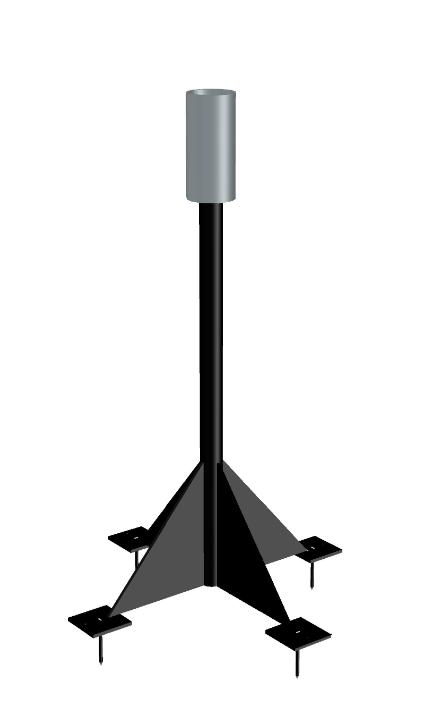
\includegraphics[height = 0.5\textheight]{buoy_stand.PNG}
	\caption{Diagram of the buoy stand for the SHARC buoy. The stand consists of stainless steel and painted mild steel to withstand the climate of the Southern Ocean and stop the stand from rusting. A cradle at the top of the stand houses the buoy and secures it to the stand via a screw. The buoy stand elevates the electronics 1 m above the ice to overcome the effects of snow growth and flooding. Finally, spikes at the bottom of the base will secure the stand to the ice floe. Drawn by R. Verrinder.}
	\label{fig:stand}
\end{figure}

\subsection{Enclosure}

The second part of the mechanical subsystem is the physical buoy enclosure, which was designed by R. Verrinder. The greatest challenge for designing this system was selecting a material that was both lightweight and low-temperature resistant. A decision was made to use High-Density Polyethylene (HDPE) which can survive temperatures up to $-120 ^\circ$ C before becoming too brittle \cite{drnovska2003surface}. The enclosure was designed to fit the housing on the buoy stand while providing ample room for the antennas of the various communication modules. It was split into three parts: A top enclosure, a bottom enclosure and a connector block. A schematic of the enclosure is shown in Figure \ref{fig:enclo_schem}
\begin{figure}[H]
	\centering
	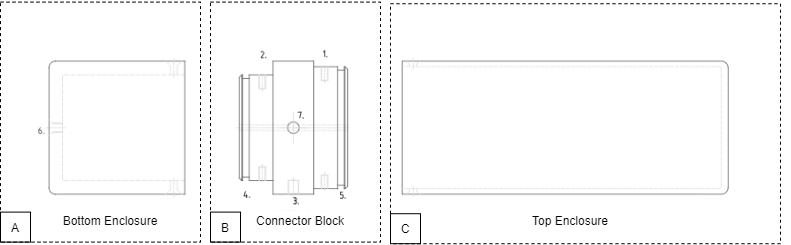
\includegraphics[width=\textwidth]{enclo_schem.PNG}
	\caption{2-D exploded view of the buoy enclosure showing (A) the bottom enclosure for the power module, (B) the connector block which also acts as a base for the electronics and (C) the top enclosure which covers the electronics. Drawn by R. Verrinder.}
	\label{fig:enclo_schem}
\end{figure}

\begin{table}[H]
	\centering
	\caption{Primary measurements of the buoy enclosure taken from the schematic in Appendix \ref{app:appendix.schem}.}
	\setlength{\extrarowheight}{5pt}
	\begin{tabular}{l  l c}
		\hline
		\textbf{Component} &   \textbf{Dimension} &   \textbf{Size [mm]} \\
		\hline
		\hline
		\setlength{\extrarowheight}{2.5pt}
		\multirow{4}{*}{Top enclosure} & Height & 240\\
		&  Outer diameter & 98  \\
		&  Wall thickness & 4 \\ 
		&  Base thickness & 5 \\
		\hline
		\multirow{3}{*}{Bottom enclosure} & Height & 100\\
		& Outer diameter & 98  \\
		& Wall and base thickness & 10 \\ 
		\hline
		\multirow{5}{*}{Connector block} & Height & 80\\
		&  Outer diameter & 98  \\
		&  Top inner diameter & 89.94  \\ 
		&  Bottom inner diameter & 77.85\\
		&  O-ring thickness & 2.6 \\
		\hline
		\hline
	\end{tabular}
	
	\label{tab:enc_meas}
\end{table}

This design allows for easy access to the electronics as well as separation between the various subsystems. The connector block acts as a connection point for the electronics in version 1 of the buoy. This point of contact was a three-dimensional printed connector for a vertically mounted printed circuit board (PCB). In version 2 of the buoy, this was replaced by a row of screw holes around the connector block to connect a horizontal stack of customised PCBs. This was found to greatly improve the robustness of the system and prevented components from breaking during transport and deployment. The communication modules, microcontroller and sensors were mounted in the top enclosure while the batteries and power system were placed in the bottom enclosure. The power system was connected to the top enclosure through a drill hole in the connector block. The system was waterproofed by placing two o-rings on either side of the connector block. The top and bottom enclosure are fastened to the connector block using a a flat head counter-sunk hex screw. Finally a drill hole in the connector block allowed the system to be secured to the buoy stand preventing it from falling out during deployment.

\section{Electronics}

The electronics for the system refer to the communication subsystems, power electronics, sensors and processors. Due to project time constraints, the approach to developing the platform was to select off-the-shelf components that satisfied the subsystem specifications shown in Table \ref{tab:sys_specs}. Further consideration was given to components that were low power (SP011, SP012) and cost effective (SP013). Additionally, devices with intelligent operations were selected as this would allow us to effectively control the current consumption and operations of the device. These consisted of components with programmable settings such as digital sensors and modems. The following section gives an overview of the selection consideration for each subsystem.

\subsection{GPS}
\label{subsec:ch3_gps}
A u-blox NEO-7M\footcite{UBLOX_M7N_DATA} GPS receiver was initially selected during the 2018 design concept phase as it was easy to procure and has a small form factor. The positioning  module was designed around a Waveshare\footcite{waveshare} development board which significantly decreases the development time. The board comes with an active patch antenna which has a gain of about 30 dB \cite{waveshare}. In addition, the component is low power with a relatively fast acquisition time and accuracy. The device also can be configured to output diagnostic information such as dilution of procession with the associated measurement which can provide a greater understanding of satellite connectivity in the region. However,  this product has been depreciated by the time the latest buoy was developed. To overcome this, we opted for the u-blox NEO-M9N\footcite{UBLOX_M9N_DATA} module which had improved performance at a higher cost. Both GPS modules are shown in Figure \ref{fig:gps_mod}.

\begin{figure}[H]
	\centering
	\begin{subfigure}[b]{0.45\textwidth}
		\begin{tikzpicture}
			\node[anchor=south west,inner sep=0] (image) at (0,0) {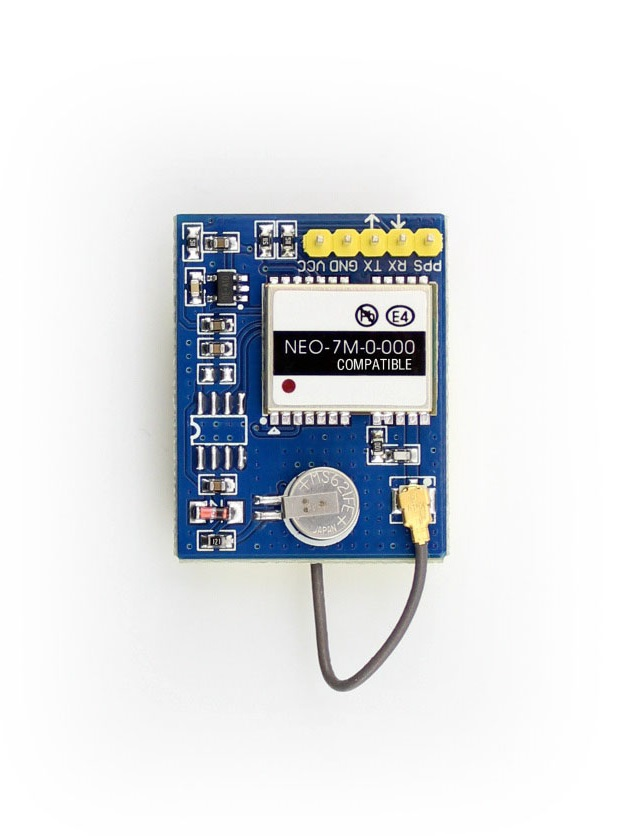
\includegraphics[width = 6cm,height=8cm]{NEO7.jpg}};
			\begin{scope}[x={(image.south east)},y={(image.north west)}]
				\draw[color=black, ultra thin,fill=white] (0.0,0.0) rectangle (0.21,0.16) node[pos=.5] {A};
			\end{scope}
		\end{tikzpicture}
	\end{subfigure}%
	\hfill
	\begin{subfigure}[b]{0.45\textwidth}
		\begin{tikzpicture}
			\node[anchor=south west,inner sep=0] (image) at (0,0) { 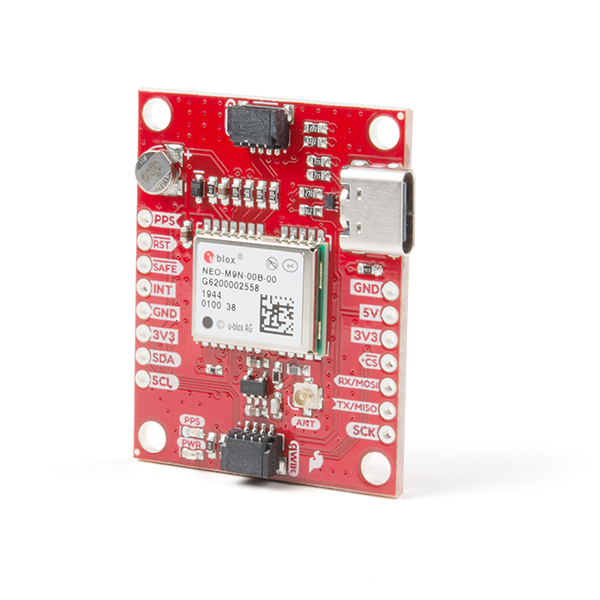
\includegraphics[width = 6cm,height=8cm]{NEO9.jpg}};
			\begin{scope}[x={(image.south east)},y={(image.north west)}]
				\draw[color=black, ultra thin,fill=white] (0.0,0.0) rectangle (0.21,0.16) node[pos=.5] {B};
			\end{scope}
		\end{tikzpicture}    
	\end{subfigure}
	\caption{ The u-blox GPS Modules selected for this project which are: (A) the u-blox NEO-7M on a Waveshare breakout board \cite{waveshare} and (B) a u-blox NEO-M9N on a Sparkfun breakout board \cite{UBLOX_M9N_DATA}.}
	\label{fig:gps_mod}
\end{figure}

Table \ref{tab:gps_mod} below shows a comparison of the two modules and their key performance parameters.

\begin{table}[H]
	\centering
	\caption{Comparison of key parameters between the initial u-blox NEO-7M GNSS module and the updated u-blox NEO-N9M module.}
	\label{tab:gps_mod}
	\setlength{\extrarowheight}{5pt}
	\begin{tabular}{l l l}
		\hline
		\textbf{Specification} & NEO-7M & EO-M9N\\
		\hline
		\hline
		Positional accuracy [m] & 2.5  & 2.0 \\
		\hline
		\multirow{3}{*}{Communication type} & UART & UART\\ & I$^2$C & I$^2$C \\ & SPI & SPI\\
		\hline
		Cold-start time [s]& 30 & 26\\
		\hline
		Supply voltage [V] & 1.65 to 3.6 & 2.7 to 3.6\\
		\hline
		Active current draw [mA] & 32 &  42\\
		\hline
		Price\tablefootnote{Price as of March 2021} & R269\tablefootnote{Source: \url{https://www.digikey.co.za/}}  & R1,195\tablefootnote{Source: \url{https://www.robotics.org.za/}}\\
		\hline
		\hline
	\end{tabular}
	\label{tab:neo7}
\end{table}

 Shows the u-blox NEO-M9N offers improved performance  over the u-blox NEO-7M at a higher cost and higher power consumption. This module comes on a Sparkfun GPS Breakout\footnote{Available at: \url{https://learn.sparkfun.com/tutorials/sparkfun-gps-neo-m9n-hookup-guide}} - NEO-M9N U.FL (Qwiic) board which optionally comes with an integrated chip antenna. The chip antenna however has a very small gain making it unsuitable to be used for this application. Therefore, an additional antenna was bought. 

\subsection{Iridium}

As discussed in Section \ref{sec:sec3_UR}, the Iridium modem is critical for ensuring data can be transmitted from remote locations where other forms of communication are unavailable. When selecting a modem, key considerations were given to the physical size, bandwidth as well as coverage. In addition, we require a module that is low powered and cost effective. For this reason, we have selected the Rock7 RockBLOCK 9603\cite{rockblock2019image} which is shown in Figure \ref{fig:rockblock} below.

\begin{figure}[H]
	\centering
	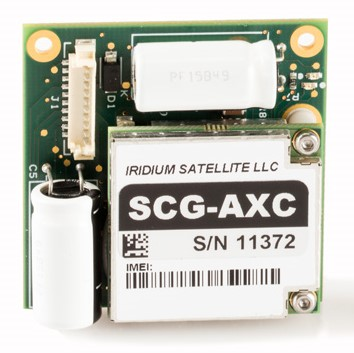
\includegraphics[width = 0.3\textwidth]{rockblock9603.jpg}
	\caption{A Rock7 RockBLOCK 9603 satellite module containing an Iridium 9603 modem \cite{9603} and a coaxial Sub-miniature version A (SMA) connector for an external antenna. Image by \textcite{rockblock2019image}.}
	\label{fig:rockblock}
\end{figure}

This module contains an Iridium 9603 modem on a specially designed power board. The device communicates via Universal Asynchronous Receiver/Transmitter (UART) with the option for flow control. Communication is performed through a ten-pin Molex PicoBlade connector. The module contains four communications pins, one digital input pin and two digital output pins. Power is supplied either through a 5 V pin or 3.3V pin in addition to the ground pin. A brief description of the pinout is given in Table \ref{tab:ir_pinout}. 

\begin{table}[H]
	\centering
	\caption{Pinout for the Rock7 RockBLOCK 9603 Iridium modem.}
	\setlength{\extrarowheight}{5pt}
	\begin{tabular}{c l l}
		\hline
		\textbf{Pin number} & \textbf{Label} & \textbf{Pin description}\\
		\hline 
		\hline
		1 & RXD & UART Output Pin \\
		
		2 & CTS & Flow control clear to send\\
		3 & RTS & Flow control request to send\\
		4 & NetAv & Network available \\
		5 & RI & Ring inidcator \\
		6 & TXD & UART input pin \\
		7 & OnOff & Sleep control\\
		8 & 5V & 5 V max supply pin \\
		9 & Li-Ion & 3.7 V max supply pin \\
		10 & GND & Ground \\
		\hline
		\hline
	\end{tabular}
	
	\label{tab:ir_pinout}
\end{table}

The device communicates via UART through the RXD and TXD pins. Additional flow control pins Clear To Send (CTS) and Request To Send (RTS) pins are available in the interface. However, these are optional. The OnOff pin can be used to put the device to sleep which significantly improves power performance. Finally, the NetAv and Ring Indicator are digital output pins that can be used to indicate whether there is sufficient signal to transmit as well as to notify when a message is waiting to be downloaded respectively.  Finally, the key characteristics for the device are shown in Table \ref{tab:ir_specsmech} to \ref{tab:ir_specscomm}.

\begin{table}[H]
	\centering
	\caption{Table showing the mechanical feature parameters of the Rock7 RockBLOCK 9603 module \cite{9603}.}
	\setlength{\extrarowheight}{5pt}
	\begin{tabular}{lc}
		\hline
		\multicolumn{2}{l}{\textbf{Mechanical features}}\\
		\hline
		\hline
		Antenna & Patch or external SMA\\
		\hline
		Temperature rating [$^\circ$ C] & -40 to 85\\
		\hline
		Dimensions [mm]  & $45.0 \times 45.0 \times 15.0$ \\
		\hline
		Price\tablefootnote{Cost as of March 2021 from \cite{rockblock2019image}} & R3,571\tablefootnote{GBP 1 = ZAR 20.41}\\
		\hline
		\hline
	\end{tabular}
	
	\label{tab:ir_specsmech}
\end{table}

\begin{table}[H]
	\centering
	\caption{Table showing the power consumption parameters of the Rock7 RockBLOCK 9603 module \cite{9603}.}
	\setlength{\extrarowheight}{5pt}
	\begin{tabular}{lc}
		\hline
		\multicolumn{2}{l}{\textbf{Power characteristics}}\\
		\hline
		\hline
		\multirow{2}{*}{Supply Voltage [V]} & 5 \\ & 3.3\\ 
		\hline
		Start-up current [mA] & 450 \\
		\hline
		Active current [mA] & 100 \\
		\hline
		Sleep current [$\mu$A] & 200\\
		\hline
		\hline
	\end{tabular}	
	\label{tab:ir_specspower}
\end{table}

\begin{table}[H]
	\centering
	\caption{Table showing the communication parameters of the Rock7 RockBLOCK 9603 module \cite{9603}.}
	\setlength{\extrarowheight}{5pt}
	\begin{tabular}{lc}
		\hline
		\multicolumn{2}{l}{\textbf{Communication}}\\
		\hline
		\hline
		Baud rate [bits/s] & 19200\\
		\hline
		Data bits &  8\\
		\hline
		Stop bits & 1 \\
		\hline
		Parity & none \\
		\hline
		Maximum upload size [bytes] & 340\\
		\hline
		Maximum download size [bytes]	 & 270\\
		\hline
		\hline
	\end{tabular}
	
	\label{tab:ir_specscomm}
\end{table}
\subsection{Environmental sensors}

Two versions of the buoy were developed from 2019 to 2020 with different sensing capabilities. The first version consisted of a Maxim Integrated DS18B20 temperature sensor \cite{DS18B20manual}. This is a low cost digital silicon temperature sensor with a small form factor that uses one-wire interface. However, in version two, this device was replaced with the Bosch Sensortech BMP280 sensor \cite{BMP280_Datasheet}. The BMP280 sensor featured pressure sensing as well as temperature sensing as well as a programmable interface. Furthermore, the BMP280 can optionally be ordered on an Adafruit BMP breakout board \cite{BMP280breakout} whereas the DS18B20 arrives as a stand-alone through-hole component that requires an additional circuit. The devices are shown in Figure \ref{fig:bmpds} while a comparison of the features of each device is given in Table \ref{tab:senv_spec}.

\begin{figure}[H]
	\centering
	\begin{subfigure}[t]{.45\textwidth}
		\begin{tikzpicture}
			\node[anchor=south west,inner sep=0] (image) at (0,0) { 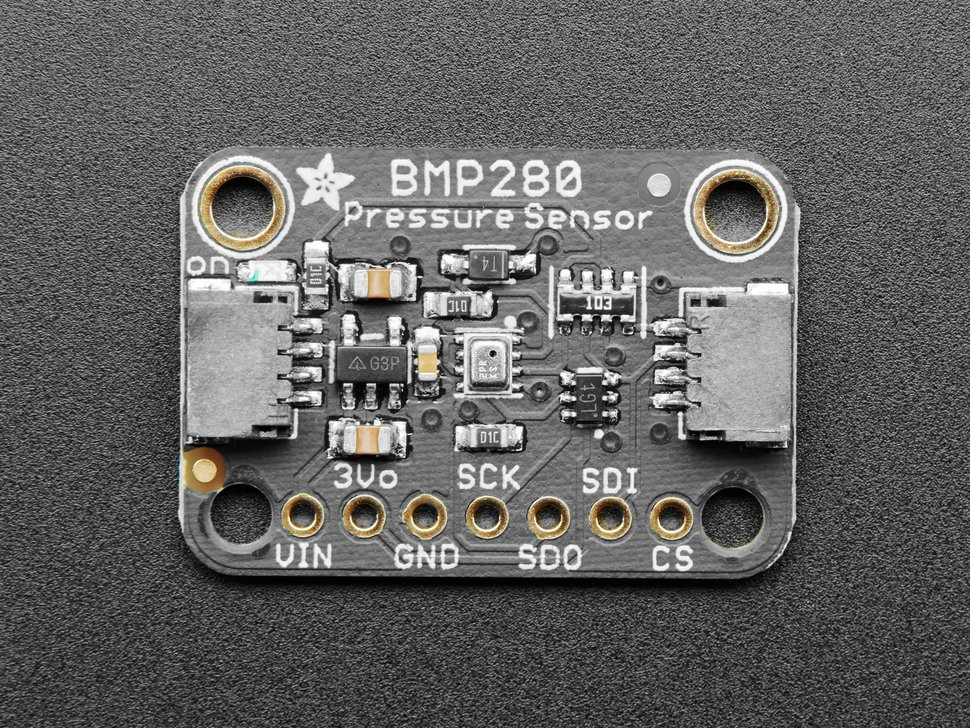
\includegraphics[width = 6cm]{BMP280.jpg}};
			\begin{scope}[x={(image.south east)},y={(image.north west)}]
				\draw[color=black, ultra thin,fill=white] (0.0,0.0) rectangle (0.21,0.16) node[pos=.5] {A};
			\end{scope}
		\end{tikzpicture}
	\end{subfigure}
	\hfill
	\begin{subfigure}[t]{.45\textwidth}
		\begin{tikzpicture}
			\node[anchor=south west,inner sep=0] (image) at (0,0) { 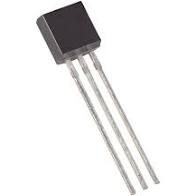
\includegraphics[width = 6cm]{ds18b20.jpg}};
			\begin{scope}[x={(image.south east)},y={(image.north west)}]
				\draw[color=black, ultra thin,fill=white] (0.0,0.0) rectangle (0.21,0.16) node[pos=.5] {B};
			\end{scope}
		\end{tikzpicture}
	\end{subfigure}
	\hfill

	\caption{ Environmental sensing devices selected for the buoy. (A) The Bosch Sensortech BMP280 digital pressure and temperature sensor on an Adafruit sensor breakout board \cite{BMP280breakout} and (B) a Maxim Integrated DS18B20 in a through hole TO-226-3 package \cite{DS18B20manual}.}
	\label{fig:bmpds}
\end{figure}

\begin{table}[H]
	\centering
	\caption{Comparison of performance between the Bosch Sensortech BMP280 and Maxim Integrated DS18B20 environmental sensors. The term "Not applicable" or N/A is given where a parameter does not apply to a device.}
	\setlength{\extrarowheight}{5pt}
	\begin{tabular}{lcc}
		\hline
		& \textbf{BMP280} & \textbf{DS18B20} \\
		\hline
		\hline
		Temperature range [$^\circ$ C ]& -40 to 85& -55 to 125 \\
		\hline
		Temperature sensor accuracy\tablefootnote{At temperatures below 0$^\circ$} [$^\circ$ C]& $\pm$1 & $\pm$ 1 \\
		\hline
		Pressure range [hPa]  & 300 to 1100 & N/A \\
		\hline
		Pressure sensor accuracy\tablefootnote{At temperatures below 0$^\circ$} [hPa] & $\pm$1.7 & N/A\\
		\hline
		Price\tablefootnote{As of March 2021 } & R47\tablefootnote{Source: \url{https://www.digikey.co.za/short/80dv2nhm}}& R77\tablefootnote{Source: \url{https://www.digikey.co.za/short/mqb0qm4j}} \\
		\hline
		\hline
	\end{tabular}
	\label{tab:senv_spec}
\end{table}

Table \ref{tab:senv_spec} shows a comparison between the Bosch Sensortech BMP280 and Maxim DS18B20 performance characteristics. The temperature ranges of both sensors are capable of measuring subzero temperatures at an accuracy of $\pm1^\circ$ C which, is required to survive in the Southern Ocean climate as discussed in Chapter \ref{ch:chapter2}. Only the BMP280 can measure temperature and pressure, whereas the DS18B20 can only measure temperature. Furthermore, the BMP280 cost R47 cheaper than the DS18B20 at R77. However, this is for the standalone BMP280. This device can be, optionally,  ordered on an Adafruit breakout board. However, this increases the price to R218\footnote{Source: \url{https://www.digikey.co.za/short/qbn473mr}}. Therefore, the BMP280 was selected for version 2 as it contains more environmental sensing features for a lower price. The power consumption characteristics of each device are shown in Table \ref{tab:env_power}.

\begin{table}[H]
	\centering
	\caption{Comparison between supply voltage and current draw of the BMP280 and DS18B20.}
	\setlength{\extrarowheight}{5pt}
	\begin{tabular}{lcc}
		\hline
		&  \textbf{BMP280} & \textbf{DS18B20}\\
		\hline
		\hline
		Supply voltage [V] & 3.0 to 5.5 & 1.7 to 3.6\\
		\hline
		Sleep current [$\mu$A]& 0.75 & 0.3\\ 
		\hline
		Active current [$\mu$A] & 4.2 &1500 \\
		\hline
		\hline

	\end{tabular}
	\label{tab:env_power}
\end{table}

Table \ref{tab:env_power} shows the power performance characteristics of the BMP280 and the DS18B20. The DS18B20 has a lower operating voltage requirement with a smaller sleep current draw than the BMP280. However, the DS18B20 has a much higher active current. Furthermore, both devices can operate at 3.3 V. Therefore, the BMP280 will have the lowest active power consumption during operation. \par 

In conclusion, the BMP280 offers both temperature and pressure sensing at a lower price than the DS18B20 that can only perform temperature measurements. Therefore the BMP280 was selected for version 2 of the buoy to increase environmental sensing capabilities.

\subsection{Power monitoring sensors}

Finally, a digital sensor for power monitoring was selected to provide constant feedback on the status of the power system. This device is used to monitor the battery voltage and current to keep track of the buoys power consumption. To achieve this, the Texas Instruments INA219A I$^\text{2}$C power monitor \cite{INA219} was selected. This device has a high reported accuracy of 1\% over a full temperature range and is fully programmable. The device  communicates via I$^2$C with 16-bit registers storing values for  current (mA), voltage (V) and power (mW). The device is extremely low power with a high voltage measurement range and on-board calibration features. The integrated circuit (IC) is shown in Figure \ref{fig:ina} while the key performance characteristics are shown in Table \ref{tab:INA_spec}.

\begin{figure}[H]
	\centering
	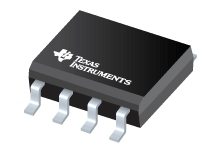
\includegraphics[width= 0.3\textwidth]{INA219.jpg}
	\caption{3-D render\protect\footnotemark of the Texas Instruments INA219 current/power monitor I$^2$C chip in an 8-pin small outline integrated circuit (SOIC) package \cite{INA219}. }
	\label{fig:ina}
\end{figure}
\footnotetext{Source: \url{https://www.ti.com/product/INA219}}

\begin{table}[H]
	\centering
	\caption{Performance specifications for the INA219 current monitor chip.}
	\setlength{\extrarowheight}{5pt}
	\begin{tabular}{l c}
		\hline
		\multicolumn{2}{l}{\textbf{Performance characteristics}}\\
		\hline
		\hline
		Operating temperature [$\degree$ C] & -40 to 125 \\
		\hline
		V$_{\text{shunt}}$ range [mV] & 40 to 320\\ 
		\hline
		\multirow{2}{*}{V$_{\text{bus}}$ range [V] } & 0 to 16\\ & 0 to 32\\
		\hline
	    ADC resolution & 12-bits\\
		\hline
		Measurement error &$\pm$1\%\\ 
		\hline
		Price\tablefootnote{Price as of March 2021}  & R16\tablefootnote{Source: \url{https://www.digikey.co.za/short/255dtrfm}}\\
		\hline
		\hline
	\end{tabular}
	
	\label{tab:INA_spec}
\end{table}

\begin{table}[H]
	\centering
	\caption{Power specifications for the INA219 current monitor chip.}
	\setlength{\extrarowheight}{5pt}
	\begin{tabular}{l c}
		\hline
		\multicolumn{2}{l}{\textbf{Power characteristics}}\\
		\hline
		\hline
		Supply voltage [V]  & 3.3 V to 5 V\\
		\hline
		Quiescent current [mA]  & 0.7 mA to 1mA\\
		\hline
		Standby current [$\mu$A] &6 to 15\\
		\hline
		\hline
	\end{tabular}
	
	\label{tab:INA_specpwr}
\end{table}

Table \ref{tab:INA_spec} above shows that the device is capable of measuring voltage, current and power at low temperatures up to -40$\degree$ C thereby making it a suitable choice for active power monitoring of the device in the polar climate.

\subsection{Inertial measurement unit}

The TDK InvenSense MPU6050\cite{mpu6050} is a 6-axis inertial measurement unit IMU that measures the acceleration and rotational velocity of 3 axes respectively. This component has a small form factor, low power and is fully programmable allowing the device to operate in different modes thereby optimising the data flow to and from the device. While the device does not contain a magnetometer, this is not an issue since the region suffers greatly from magnetic distortion \cite{kohout2015device} thereby rendering all magnetic readings to be unreliable. In addition, the acceleration of waves can be defined by Stoke's upper limit as 0.5 g for a non breaking wave  \cite{kohout2015device}. The device has a programmable full scale range for both the accelerometer and gyroscope. It contains an infinite impulse response (IIR) filter and on-board self testing for added robustness and data integrity thereby making it  the ideal device for this application. The device can be, optionally, ordered on a SparkFun Triple Axis Accelerometer and Gyro Breakout - MPU-6050 which is shown in Figure \ref{fig:mpubreakout}. The key parameters for the device are shown in Table \ref{tab:mpu_specscc} to \ref{tab:mpu_specs}.

\begin{figure}[H]
	\centering
	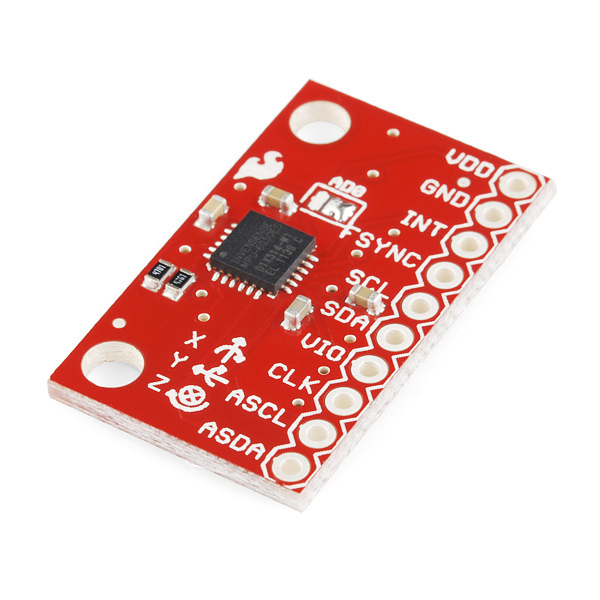
\includegraphics[width = 0.3\textwidth]{mpu6050 breakout.jpg}
	\caption{A TDK Invensense MPU6050 6 degrees of freedom inertial measurement unit on a Sparkfun development board. The board allows for fast prototyping with communication performed via I$^2$C. Image source: \cite{mpu6050breakout}.}
	\label{fig:mpubreakout}
\end{figure}

\begin{table}[H]
	\centering
	\caption{Performance characteristics of the TDK Invensense MPU6050 6-axis inertial measurement unit (IMU) showing the accelerometer performance. }
	\setlength{\extrarowheight}{5pt}
	\begin{tabular}{lc}
		\hline
		\multicolumn{2}{l}{\textbf{Accelerometer}}\\
		\hline
		\hline
		Full scale resolution [g] & $ \pm\text{2 to } \pm\text{8}$\\
		\hline
		Sensitivity [$\mu$g/LSB ] &  61.17 to 488.281\\
		\hline
		Sample rate [Hz] & 4 to 1000\\
		\hline
		Noise performance [$\mu g/\sqrt{Hz}$] & 400\\
		\hline
		\hline
	\end{tabular}
	\label{tab:mpu_specscc}
\end{table}

\begin{table}[H]
	\centering
	\caption{Performance characteristics of the TDK Invensense MPU6050 6-axis inertial measurement unit (IMU) showing the gyroscope performance. }
	\setlength{\extrarowheight}{5pt}
	\begin{tabular}{lc}
		\hline
		\multicolumn{2}{l}{\textbf{Gyroscope}}\\
		\hline
		\hline
		Full scale resolution [$\degree/s$]  & $\pm \text{250 to } \pm \text{2000}$ \\
		\hline
		Sensitivity [$(\mu\degree/s)/LSB^{-1}$]&  7.63 to 60.98\\
		\hline
		Sample rate [Hz] & 4 to 8000\\
		\hline
		Noise performance [$(\mu\degree/s)/\sqrt{Hz}$] & 0.005\\
		\hline
		\hline
	\end{tabular}
	\label{tab:mpu_specsgyro}
\end{table}

\begin{table}[H]
	\centering
	\caption{Performance characteristics of the TDK Invensense MPU6050 6-axis inertial measurement unit (IMU) showing the device temperature rating, power consumption and price. }
	\setlength{\extrarowheight}{5pt}
	\begin{tabular}{lc}
		\hline
		\multicolumn{2}{l}{\textbf{Device characteristics}}\\
		\hline
		\hline
		Temperature range [$\degree$ C] & -40 to 85\\
		\hline
		Low pass filter range [Hz] & 5 to 256 \\
		\hline
		Supply voltage [V] & 2.4 to 3.5\\
		\hline 
		Maximum active current [mA] & 3.9\\
		\hline
		Low power mode current\tablefootnote{for output data rate (ODR) < 5 Hz} [$\mu$A]: & 20 \\
		\hline
		Price\tablefootnote{Price as of March 2021}: & R110\tablefootnote{Source: \url{https://www.digikey.co.za/short/rh95nm3v}}\\
		\hline
		\hline
	\end{tabular}
	\label{tab:mpu_specs}
\end{table}



Table \ref{tab:mpu_specs} shows that the TDK InvenSense MPU6050 IMU has the capabilities to measure acceleration and angular velocity necessary to perform wave calculations as described in Chapter \ref{subsec:ch2_wavemeas}. The device can operate with a voltage supply of 2.4 V to 3.5 V. Furthermore, the lowest sample rate of the IMU is 4 Hz which is well above the Nyquist sampling criteria for open ocean waves as discussed by \textcite{earle1996nondirectional} in Subsection \ref{subsec:ch2_wavemeas}. This device is also capable of operating in low temperatures up to -40$\degree$ C which, is suitable for the Southern Ocean climate. The chip can, optionally, arrive on a  SparkFun Triple Axis Accelerometer and Gyro Breakout - MPU-6050. However, this board has an increased cost of R437\footnote{Source: \url{https://www.digikey.co.za/short/bpqqdjdv}} compared to R110 for a standalone chip. For this reason, the Sparkfun board was used to develop and test the firmware for the device. Verrinder and Pead designed the circuit for the MPU6050 for the final version of the buoy.

\subsection{Memory}
\label{subsec:ch3_mem}
Physical memory is an important feature in the device as it allows for permanent storage of data during the life cycle of buoy. Having the device in various sleep modes may result in lost data if the data are stored in non-volatile memory.

Flash chips were selected as a permanent solution. A total of four Adesto Technologies AT45DB641E SPI serial flash chips \cite{AT45DB641E} were selected and mounted on a PCB directly interfacing with the system. Each chip can hold up to 64 megabits of data. Data can be read/written at speeds of up to 85 MHz of 15 MHz in low power mode. These chips are low power with high data retention requiring a supply voltage of 1.7 V to 3.6 V and draws a maximum of 11 mA in active read mode thereby making it one of the lowest power consumption components in the system. In addition, the device comes with two 256 byte buffers that can store data while a read/write operation is taking place. Memory is Organised into sectors (2 to 256 KB long), blocks (2 KB long) and pages (256 bytes) with write, read and erase options at each level. The device comes in a surface mount package shown in Figure \ref{fig:flashAAHAH}. Table \ref{tab:flash_specs} shows key performance characteristics.

\begin{figure}[H]
	\centering
	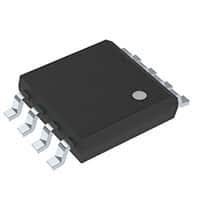
\includegraphics[width = 0.3\textwidth]{AT45DB.jpg}
	\caption{The Adesto Technologies SPI serial flash chips in a surface mount package. Image source: \cite{flashchipimage}.}
	\label{fig:flashAAHAH}
\end{figure}
\begin{table}[H]
	\centering
	\caption{Key performance characteristics for the AT45DB641E flash chips \cite{AT45DB641E} including temperature rating, power consumption, storage capacity and price.}
	\setlength{\extrarowheight}{5pt}
	\begin{tabular}{lc}
		\hline
		\textbf{Performance characteristics} &\\
		\hline
		\hline
		Operating temperature [$\degree$ C]  &  -40 to 85 \\
		\hline
		Storage capacity [Mbit] & 64 \\
		\hline
		Supply voltage [V]    & 1.7 to 3.6\\
		\hline
		Standby current [$\mu$A] & 45 \\
		\hline
		Active current [mA]  & 22 \\
		\hline
		Price   & R65\tablefootnote{Source: \url{https://za.rs-online.com/}}\\
		\hline
		\hline
	\end{tabular}
	\label{tab:flash_specs}
\end{table}

\subsection{Processor}

For the processor, a single processing unit was selected to reduce complexity of the system. However, to satisfy the requirements for the buoy, a processor must be selected with sufficient peripheral ports to handle communication from all sensors, communication modules and memory banks. In addition, there should be sufficient digital input and output pins to control the sensors and provide feedback. The communication peripheral requirements are condensed into Table \ref{tab:micro_ports}: 

\begin{table}[H]
	\centering
	\caption{ Type and number of communication ports to facilitate communication among all the external modules.}
	\setlength{\extrarowheight}{5pt}
	\begin{tabular}{lc}
		\hline 
		\textbf{Peripheral name} & \textbf{Qty }\\
		\hline \hline
		UART & 2\\
		\hline
		I$^2$C & 2\\
		\hline
		SPI & 2\\
		\hline
		Digital pins & 11\\
		\hline 
		\hline
	\end{tabular}
	\label{tab:micro_ports}
\end{table}

From Subsections \ref{subsec:ch3_gps} to \ref{subsec:ch3_mem}, the modules given have a data requirement and a communication requirement. Some modules, such as the RockBLOCK 9603 modem, require additional digital pins. Furthermore, all sensors output data at different resolutions. The BMP280 and MPU6050 have an 8-bit resolution, while the INA219 has a 16-bit resolution. Therefore, the selected processor needs to have sufficient width to accommodate incoming data of varying sizes while containing sufficient peripherals to interface with and control the subsystems. For this reason, a 32-bit microcontroller was selected for the processing system. During the prototyping period, three processors were selected from the STMicroelectronics STM32 range of microcontrollers for different versions of the buoy. These microcontrollers are shown in Figure \ref{fig:mcus}.


\begin{figure}[H]
	\centering
	\begin{subfigure}[t]{.5\textwidth}
		\begin{tikzpicture}
			\node[anchor=south west,inner sep=0] (image) at (0,0) { 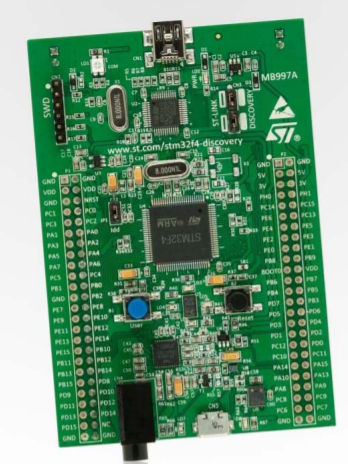
\includegraphics[width = 0.6\textwidth]{stm32f4disc.png}};
			\begin{scope}[x={(image.south east)},y={(image.north west)}]
				\draw[color=black, ultra thin,fill=white] (0.0,0.0) rectangle (0.21,0.16) node[pos=.5] {A};
			\end{scope}
		\end{tikzpicture}
	\end{subfigure}
	\hfill
	\begin{subfigure}[t]{.49\textwidth}
		\begin{tikzpicture}
			\node[anchor=south west,inner sep=0] (image) at (0,0) { 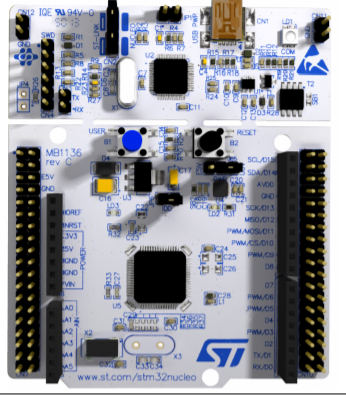
\includegraphics[width = 0.6\textwidth]{stm32f4nuc.PNG}};
			\begin{scope}[x={(image.south east)},y={(image.north west)}]
				\draw[color=black, ultra thin,fill=white] (0.0,0.0) rectangle (0.21,0.16) node[pos=.5] {B};
			\end{scope}
		\end{tikzpicture}
	\end{subfigure}
	\hfill
	\caption{The 32-bit microcontrollers used for the different versions of SHARC buoy. (A) is the STMicroelectronics STM32F407VTG6 \cite{stmdisc} on a 100-pin Discovery development board which was used for version one. (B) is the 64-pin STMicroelectronics Nucleo development board which initially contained an STMicroelectronics STM32F446RE \cite{stm32nucleo} for version 2. However, it was replaced with an STMicroelectronics STM32L476RG \cite{stm32l4} for the final version.}
	\label{fig:mcus}
\end{figure}

The first version of the buoy contained the STMicroelectronics STM32F407VGT6 \cite{stmdisc} which is available on a 100-pin Discovery development board. However, this device was found to have more peripherals than necessary and had a large power requirement. Therefore the device was replaced by the STMicroelectronics STM32F446RE \cite{stm32nucleo}. This device came on the STMicroelectronics Nucleo development board and had reduced peripherals and more optimal performance. The final processor selected was the STMicroelectronics STM32L476RG \cite{stm32l4}. Development boards were selected for the prototyping phase as they were quick to set up and program. In Figure \ref{fig:mcus}, both the Discovery and the Nucleo have pinheaders allowing for quick interfacing with the peripherals of the microcontroller. Which matched the STM32F446RE in pinout and number of peripherals. However, it was more optimised for low power operation. This microcontroller had additional wake-up pins and lower current consumption. Furthermore, the Nucleo boards have an on-board STLink debugger to program the microcontroller. However, this can be removed to reduce the physical size of the module. The STM32L476RG can be configured to detect brownout events and low power events. This provides critical feedback regarding the device's performance. Some key performance parameters of the STM32L476RE are shown in Table \ref{tab:stm_specelec} to \ref{tab:stm_speccom} .

\begin{table}[H]
	\centering
	\caption{Electrical parameters and power consumption characteristics for the STM32L476RG microcontroller. }
	\setlength{\extrarowheight}{5pt}
	\begin{tabular}{l  c}
		\hline
		\multicolumn{2}{l}{\textbf{Electrical characteristics}}\\
		\hline
		\hline
		Input voltage [V]    & 1.7 to 3.6\\
		\hline
		Active current [$\mu$A/Hz]    & 100 \\
		\hline
		Shutdown mode current [nA]  &  30 \\
		\hline
		Standby mode current [nA] &  420 \\
		\hline
		$V_{\text{brownout}}$ threshold [V] &  1.7 to 2.9\\
		\hline
		\hline
		
	\end{tabular}
	
	\label{tab:stm_specelec}
\end{table}
\begin{table}[H]
	\centering
	\caption{Processing characteristics and parameters for the STM32L476RG microcontroller. }
	\setlength{\extrarowheight}{5pt}
	\begin{tabular}{l  c}
		\hline
		\multicolumn{2}{l}{\textbf{Processor characteristics}}\\
		\hline
		\hline
		Processor   &  Arm Cortex-M4 \\
		\hline
		Processor size   & 32-bit\\
		\hline
		Float representation & Hardware FPU \\
		\hline
		Flash memory size [MB] & 1\\
		\hline
		Volatile memory (RAM) size [KB] & 128\\
		\hline
		\multirow{5}{*}{Input clock sources } & \multicolumn{1}{l}{Low speed external (LSE)}\\&  \multicolumn{1}{l}{High speed external (HSE)}\\ &  \multicolumn{1}{l}{Low speed internal (LSI)}\\ &  \multicolumn{1}{l}{Mixed speed internal (MSI)}\\ &  \multicolumn{1}{l}{High speed internal (HSI)} \\
		\hline
		Input clock frequency [MHz] & 4 to 80 \\
		\hline
		Dhrystone Benchmark: & 1.25 DMIPS/Hz \\
		\hline
		\hline
	\end{tabular}
	
	\label{tab:stm_specproc}
\end{table}

\begin{table}[H]
	\centering
	\caption{Communication ports and specifications for the STM32L476RG microcontroller. }
	\setlength{\extrarowheight}{5pt}
	\begin{tabular}{l  c}
		\hline
		\multicolumn{2}{l}{\textbf{Communication ports}} \\
		\hline
		\hline
		Total communication ports & 20 \\
		\hline
		UART ports & 5 \\
		\hline
		I$^2$C ports & 3 \\
		\hline
		SPI Ports & 3 \\
		\hline
		\hline
	\end{tabular}
	
	\label{tab:stm_speccom}
\end{table}

Tables \ref{tab:stm_specelec} to \ref{tab:stm_speccom} show the performance characteristics of the STM32L476RG. It features seven general purpose timers as well as two advanced timers and two low power timers. In addition, the device has five wake up pins which allow the device to be woken up from deep sleep (shutdown) via an external source. The device is capable of  digital siganl processing (DSP) using external libraries provided by the manufacturer. This allows the device to perform wave spectra calculations as described by \textcite{kuik1988method} and \textcite{earle1996nondirectional}. Furthermore, the STM32L4 Nucleo board contains an onboard real-time clock (RTC) with a 32.768 kHz LSE crystal to provide an accurate reference for time-based applications thereby making it the ideal component to be a processor for the buoy.

\subsection{Power electronics}

Based on the aforementioned hardware selection, the following power requirements are outlined in Table\ref{tab:pow_budget}.

\begin{table}[H]
	\centering
	\caption{Current consumption of various components as well as the estimated maximum possible current draw.}
	\setlength{\extrarowheight}{5pt}
	\begin{tabular}{l c c l}
		\hline
		\textbf{Device name} & \textbf{Qty} &  \textbf{Supply voltage [V]} & \textbf{Opperating current [mA]}\\
		\hline
		\hline
		u-blox NEO-M9N & 1 & 3.3 & 42 \\
		\hline
		Rock7 RockBLOCK 9603 & 1 & 5 &  450\\
		\hline
		Bosch Sensortech BMP280 & 1 & 3.3 & 0.0042\\
		\hline
		Texas Instruments INA219A & 1 & $V_{Bat}$\tablefootnote{INA219A supply voltage is fixed to the reference power supply \cite{INA219}} & 1\\
		\hline
		TDK Invensense MPU6050 & 1 & 3.3 & 3.9\\
		\hline 
		Adesto Technologies AT45DB641E & 4 & 3.3 & 88\\
		\hline
		STMicroelectronics STM32L476RG & 1 & 5 & 2.6\\
		\hline
		\hline
		\cline{4-4}
		\multicolumn{2}{r}{} &\multicolumn{1}{r}{\textbf{total [mA] }} & \multicolumn{1}{l}{587.50} \\
		\cline{4-4}
		\cline{4-4}
	\end{tabular}
	
	\label{tab:pow_budget}
\end{table}

From Table \ref{tab:pow_budget}, a maximum current draw of 587.50 mA can be expected if all the sensors are running concurrently. The largest consumer of power is the RockBLOCK 9603 which can draw up to 450 mA when charging. Therefore, the power supply needs to be to supply at least 500 mA during startup. Current can be conserved by placing the devices into sleep mode which further reduces the current consumption from the batteries. These techniques will be discussed in Chapter \ref{ch:ch5}. Finally, by only turning the components on when required, more power can be conserved. \par 

Therefore, a regulator is required to supply the required current at a constant voltage while being able to stand the drastic changes in current consumption. A decision was made to use a 5 V low dropout regulator (LDO) to supply the 5 V components directly. The 3.3 V components are powered through the STMicroelectronics Nucleo-L476RG on-board 3.3 V regulator. The 5 V LDO is a Texas Instruments LP3876 7 V LDO \cite{LP3876} which is shown in Figure \ref{fig:lp3876}.


\begin{figure}[H]
	\centering
	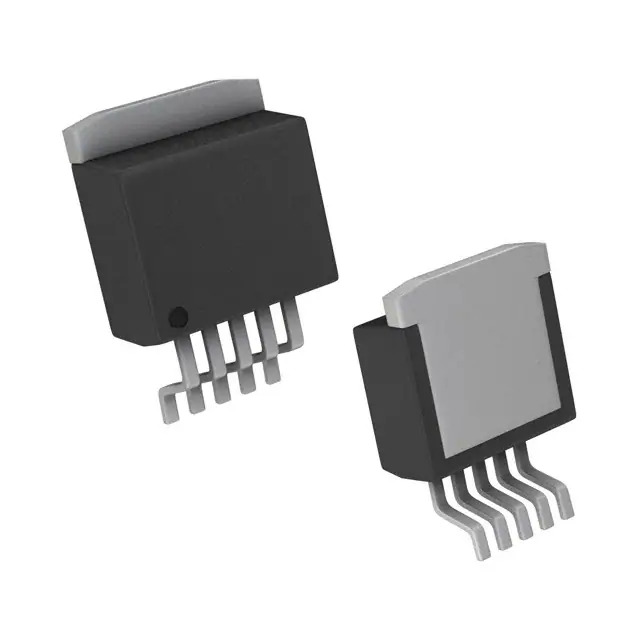
\includegraphics[width= 0.5\textwidth]{LP3876.jpg}
	\caption{3-D render\tablefootnote{Image source:\url{https://www.digikey.co.za/short/d95btr8d}} of the Texas Instruments LP3876 linear low drop out regulator in a 5-Pin DDPAK/TO-263 surface mount package \cite{LP3876}. }
	\label{fig:lp3876}
\end{figure}

This regulator is capable of supplying up to 3 A. The device has a quick response to step changes and an adjustable output voltage thereby making it the ideal device to supply power.$10$ $\mu$C tantalum capacitors are used as decoupling capacitors to filter the power source as these capacitors have excellent robustness and transient responses especially at low temperatures. Some key characteristics for the device are given in Table \ref{tab:lp_spec}.

\begin{table}[H]
	\centering
	\caption{Key performance characteristics for the Texas Instruments LP3876 linear low dropout regulator \cite{LP3876}.}
	\setlength{\extrarowheight}{5pt}
	\begin{tabular}{lc}
		\hline
		\textbf{Performance characteristics} & \\
		\hline \hline
		Input voltage [V] & 2.5 to 7.0  \\
		\hline
		Voltage regulation over current& 0.14\%\\
		\hline
		Dropout voltage at 3 A [V] & 0.8 to 1.2  \\
		\hline
		Quiescent current at 3 A  [mA]&  14\\
		\hline
		Temperature Range [$\degree$ C] &-40 to 125\\
		\hline
		Price\tablefootnote{Price as of February 2021} & R86\tablefootnote{Source: \url{https://www.digikey.co.za/short/d95btr8d}}\\
		\hline
		\hline
	\end{tabular}    
	\label{tab:lp_spec}
\end{table}



The LDO was placed on a customised PCB designed by Verrinder with the Texas Instruments INA219A current sensor as well as an indicator LED to show that the batteries have sufficient charge. The power board was supplied by 3.6 V C-cell LiSOCl$_2$ batteries. These batteries have ideal low temperature characteristics as well as a high capacity. Two cells were placed in series to create a 7.2 V power source which was placed in parallel with another 7.2 V array to increase the capacity. The batteries, battery holders and power board are connected to form a single subsystem which was placed in the bottom enclosure and connected to the microcontroller via a 7-pin cable.

\section{Final assembly}
\label{sec:ch3_final_assembly}

The final electronics choice and configurations are shown in Figure \ref{fig:sharc_final}.

\begin{landscape}
	\centering
	\vspace*{\fill}
	\begin{figure}[htpb]
		\centering
		\captionsetup{font=footnotesize}
		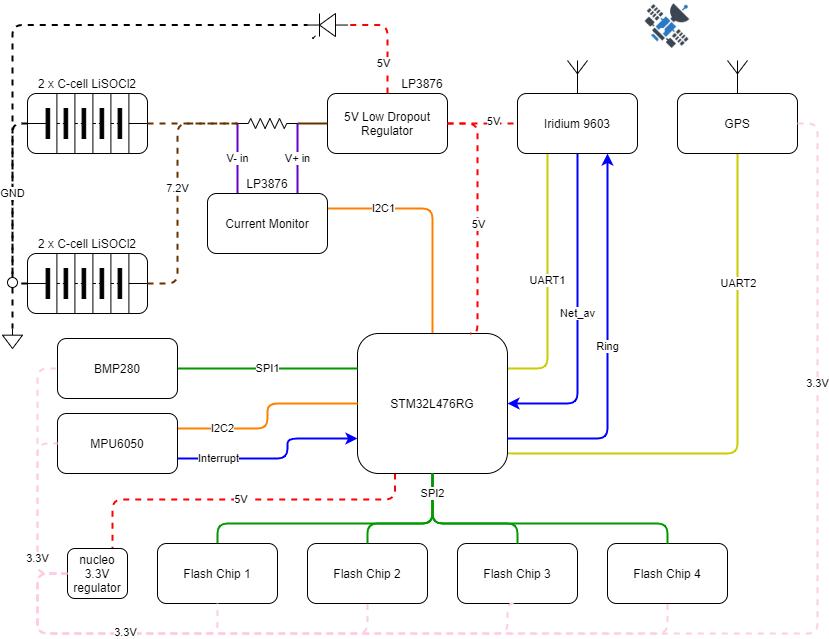
\includegraphics[height=0.6\textwidth,width=1.2\textheight]{figs/SHARC_Final.png}
		\caption{Simplified schematic of the final version of SHARC buoy showing (dash) power supply, (solid) communication and digital (arrows) connections. Also shown in the figure are lines indicating: (black) ground, (red) 5 V power, (pink) 3.3 V power, (Purple) analog inputs, (orange) I$^2$C, (yellow) UART, (green) SPI and (blue) digital input/output.}
		\label{fig:sharc_final}
	\end{figure}
	\vfill
\end{landscape}


A final costing of the system is provided in Table \ref{tab:total_cost}.
\begin{table}[H]
	\centering
	\caption{Approximate procurement cost for a single SHARC buoy node.}
	\setlength{\extrarowheight}{5pt}
	\begin{tabular}{l c r r}
		\hline \hline
		\textbf{Component name} & \textbf{Qty} & \textbf{Unit cost} & \textbf{Total}  \\
		\hline \hline
		Buoy enclosure and stand  & 1 & R1,206.84 & R1,206.84 \\
		u-blox Neo-M9N & 1 &  R1,195.45 &R1,195.45\\
		Rock7 Rockblock 9603 & 1 & R3,278.144 & R3,278.144 \\
		M1621HCT Helical Antenna & 1 & R1,411.15 & R1,411.15 \\
		BMP280 & 1 & R46.00 & R46.00 \\
		INA219A & 1 & R17.77 & R17.77 \\
		MPU6050 & 1 & R40.00 & R40.00 \\
		AT45DB641E & 4 & R65.307 & R261.229 \\
		Nucleo-l476RG & 1 & R215.98 & R215.98 \\
		Fanso C-cell 9000mAh Battery & 4 & R101.81 & R407.24 \\
		BHC-2ND Battery Holder & 4 & R61.87 & R247,48 \\
		LP3876 5V regulator & 1 & R95.19 & R95.19 \\
		Wiring and Connectors & - & R136.46 & R136.46 \\
		\hline 
		\hline
		& & \textbf{ Grand total } & R8,421.13\\ 
		\hline \hline
	\end{tabular}
	\label{tab:total_cost}
\end{table}

Customised PCBs were designed to connect the various subsystems together. The device was kept modular by separating PCBs and grouping devices by functionality. A circuit board was created for the LP3876 LDO and INA219 current sensor which was affixed to four C-cell battery holders.The battery holders have leads which were were arranged in a 2-series, 2-parallel configuration.

\begin{figure}[H]
	\centering
	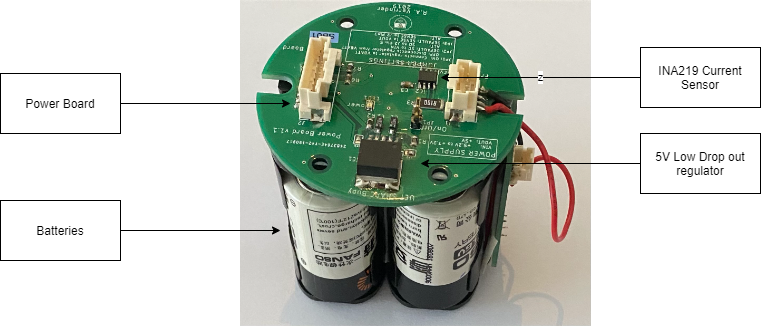
\includegraphics[scale = 0.5]{bot_encl.png}
	\caption{Power module for the SHARC BUOY. A custom PCB with a low dropout regulator and current sensor connected to a battery pack.}
	\label{fig:bot_elec}
\end{figure}

This module was placed in the bottom enclosure and fastened to the connector block using a hex screw. A customised 7-pin Molex DuraClik cable connects the module to the modules in the top enclosure. A main connector board was developed with Molex DuraClik connections for each of the aforementioned devices. The board contains two 2x16 female header rows to fit the morpho connectors of the Nucleo-L476RG development board. Two more disc-shaped PCBs were developed with the first for a communication board containing a 4-pin female header to connect the u-blox NEO GPS module and two brackets to mount the RockBLOCK 9603 Iridium module vertically. A helical antenna connects to an SMA antenna on the Iridium module. The second board was developed as a sensor board for the IMU and environmental sensor. The boards were connected in a stack configuration and fastened to the connector block using M6 metal hex spaces with the communication board being placed at the top for direct line of sight with satellites. The environmental board was secured to the base of the connector block with the BMP280 placed face-down over a hole drilled through the connector block allowing it to interface with the environment. Figure \ref{fig:top_elec} shows the configuration of the PCBs in the top enclosure of the buoy.
\begin{figure}[H]
	\centering
	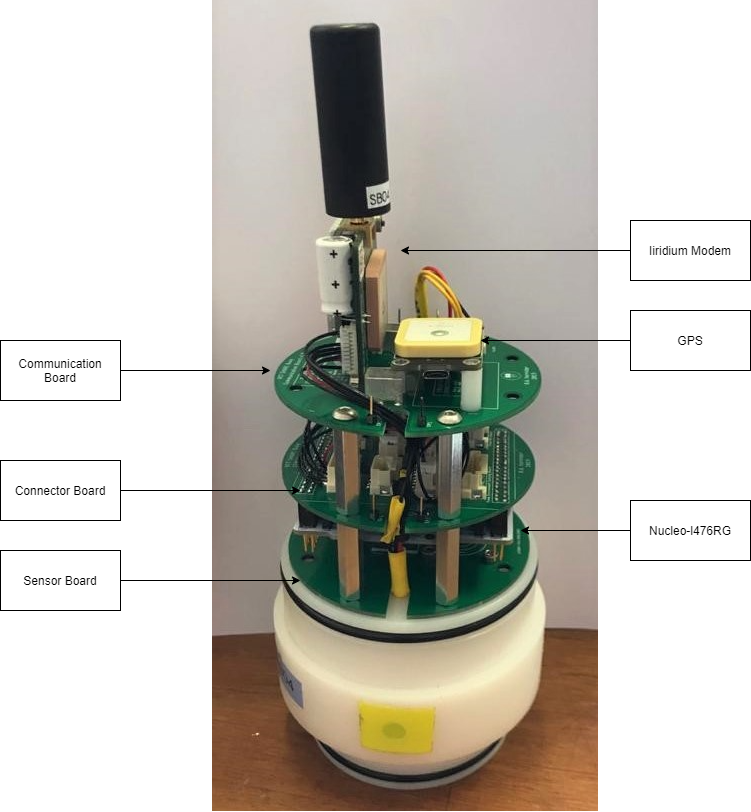
\includegraphics[scale =0.5]{Top_encl.png}
	\caption{Electronic PCB stack for the top module consisting of connector board, microcontroller board and sensor board attached to the connector block. }
	\label{fig:top_elec}
\end{figure}

This configuration greatly increases the robustness of the electronics and can overcome breaking caused by poor handling or improper deployment.  The top enclosure is placed over the electronics and fastened to the connector block using hex screws. Finally, the system is placed in the stand housing and secured using another hex screw. Final assembly of the buoy can be seen in Figure \ref{fig:sharc_final}.

\section{Conclusion}

In conclusion, this chapter outlined the construction of the SHARC buoy remote sensing device. Electronic components were selected and arranged into a system and connected together on customised PCB. This platform was then used to develop the firmware which will be discussed in the next chapter.

